% Created by tikzDevice version 0.12 on 2019-01-16 14:48:28
% !TEX encoding = UTF-8 Unicode
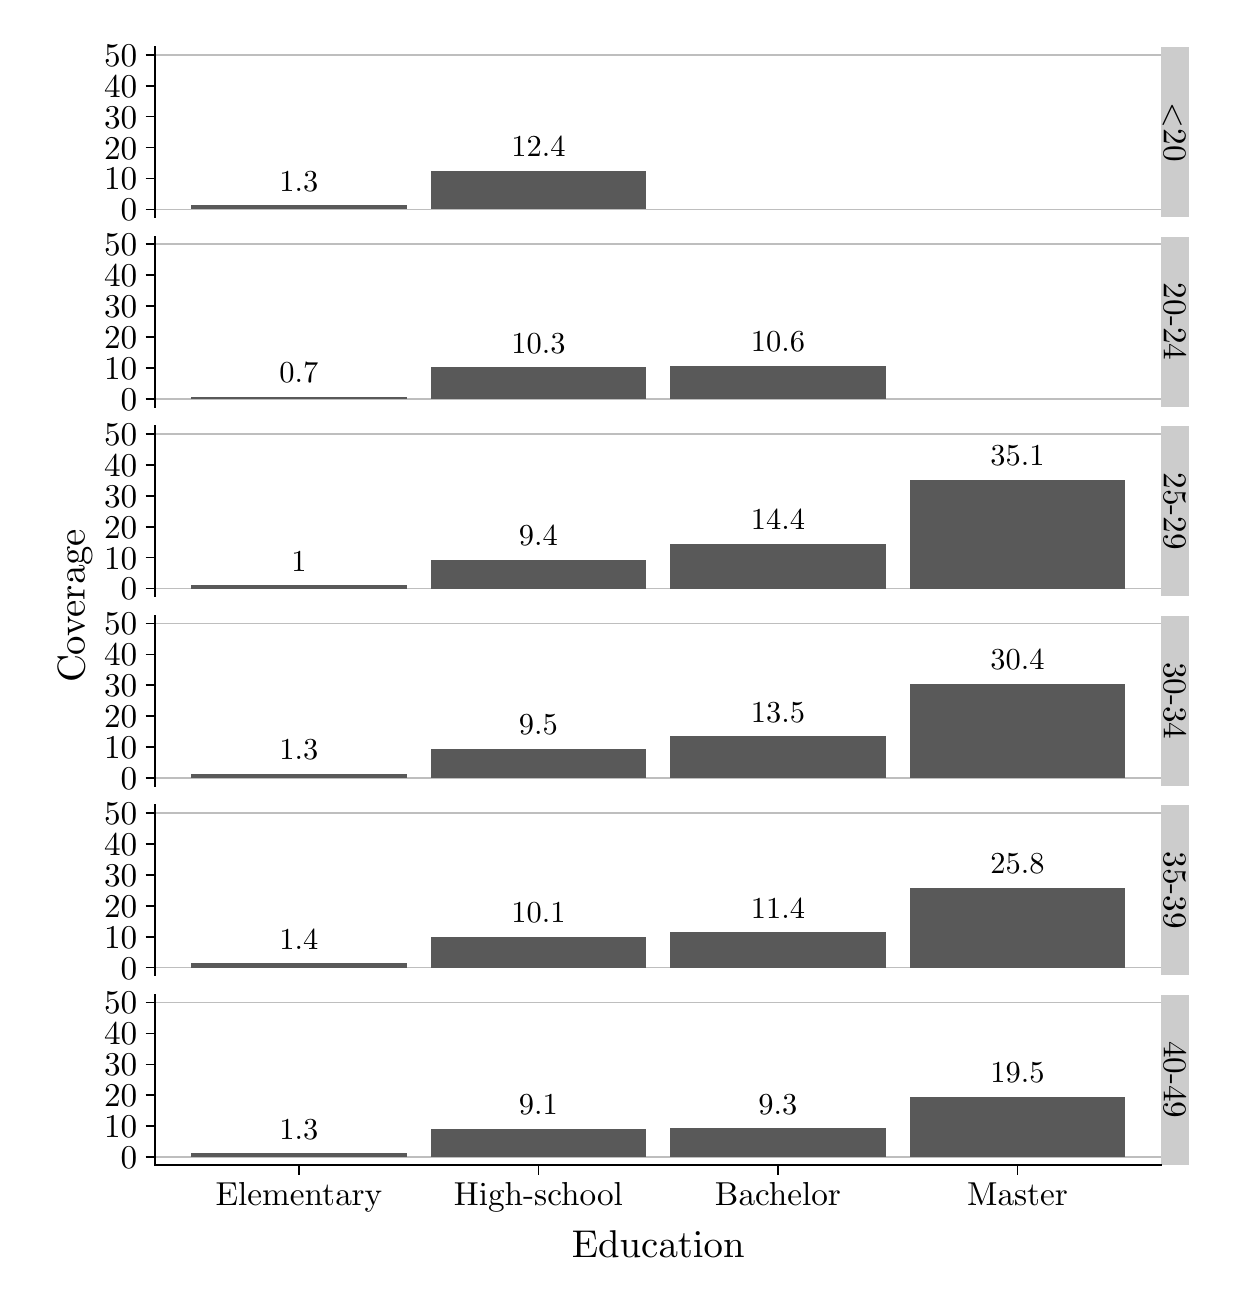
\begin{tikzpicture}[x=1pt,y=1pt]
\definecolor{fillColor}{RGB}{255,255,255}
\path[use as bounding box,fill=fillColor,fill opacity=0.00] (0,0) rectangle (426.79,455.24);
\begin{scope}
\path[clip] ( 46.08,386.75) rectangle (409.58,448.24);
\definecolor{drawColor}{RGB}{190,190,190}

\path[draw=drawColor,line width= 0.6pt,line join=round] ( 46.08,445.45) -- (409.58,445.45);

\path[draw=drawColor,line width= 0.6pt,line join=round] ( 46.08,389.55) -- (409.58,389.55);
\definecolor{fillColor}{gray}{0.35}

\path[fill=fillColor] ( 59.06,389.55) rectangle (136.96,391.04);

\path[fill=fillColor] (145.61,389.55) rectangle (223.50,403.38);
\definecolor{drawColor}{RGB}{0,0,0}

\node[text=drawColor,anchor=base,inner sep=0pt, outer sep=0pt, scale=  1.10] at ( 98.01,396.18) {1.3};

\node[text=drawColor,anchor=base,inner sep=0pt, outer sep=0pt, scale=  1.10] at (184.56,408.52) {12.4};
\end{scope}
\begin{scope}
\path[clip] ( 46.08,318.26) rectangle (409.58,379.75);
\definecolor{drawColor}{RGB}{190,190,190}

\path[draw=drawColor,line width= 0.6pt,line join=round] ( 46.08,376.96) -- (409.58,376.96);

\path[draw=drawColor,line width= 0.6pt,line join=round] ( 46.08,321.06) -- (409.58,321.06);
\definecolor{fillColor}{gray}{0.35}

\path[fill=fillColor] ( 59.06,321.06) rectangle (136.96,321.87);

\path[fill=fillColor] (145.61,321.06) rectangle (223.50,332.53);

\path[fill=fillColor] (232.16,321.06) rectangle (310.05,332.96);
\definecolor{drawColor}{RGB}{0,0,0}

\node[text=drawColor,anchor=base,inner sep=0pt, outer sep=0pt, scale=  1.10] at ( 98.01,327.01) {0.7};

\node[text=drawColor,anchor=base,inner sep=0pt, outer sep=0pt, scale=  1.10] at (184.56,337.68) {10.3};

\node[text=drawColor,anchor=base,inner sep=0pt, outer sep=0pt, scale=  1.10] at (271.11,338.10) {10.6};
\end{scope}
\begin{scope}
\path[clip] ( 46.08,249.77) rectangle (409.58,311.26);
\definecolor{drawColor}{RGB}{190,190,190}

\path[draw=drawColor,line width= 0.6pt,line join=round] ( 46.08,308.47) -- (409.58,308.47);

\path[draw=drawColor,line width= 0.6pt,line join=round] ( 46.08,252.56) -- (409.58,252.56);
\definecolor{fillColor}{gray}{0.35}

\path[fill=fillColor] ( 59.06,252.56) rectangle (136.96,253.67);

\path[fill=fillColor] (145.61,252.56) rectangle (223.50,263.06);

\path[fill=fillColor] (232.16,252.56) rectangle (310.05,268.61);

\path[fill=fillColor] (318.71,252.56) rectangle (396.60,291.83);
\definecolor{drawColor}{RGB}{0,0,0}

\node[text=drawColor,anchor=base,inner sep=0pt, outer sep=0pt, scale=  1.10] at ( 98.01,258.81) {1};

\node[text=drawColor,anchor=base,inner sep=0pt, outer sep=0pt, scale=  1.10] at (184.56,268.20) {9.4};

\node[text=drawColor,anchor=base,inner sep=0pt, outer sep=0pt, scale=  1.10] at (271.11,273.75) {14.4};

\node[text=drawColor,anchor=base,inner sep=0pt, outer sep=0pt, scale=  1.10] at (357.65,296.97) {35.1};
\end{scope}
\begin{scope}
\path[clip] ( 46.08,181.28) rectangle (409.58,242.77);
\definecolor{drawColor}{RGB}{190,190,190}

\path[draw=drawColor,line width= 0.6pt,line join=round] ( 46.08,239.97) -- (409.58,239.97);

\path[draw=drawColor,line width= 0.6pt,line join=round] ( 46.08,184.07) -- (409.58,184.07);
\definecolor{fillColor}{gray}{0.35}

\path[fill=fillColor] ( 59.06,184.07) rectangle (136.96,185.47);

\path[fill=fillColor] (145.61,184.07) rectangle (223.50,194.66);

\path[fill=fillColor] (232.16,184.07) rectangle (310.05,199.20);

\path[fill=fillColor] (318.71,184.07) rectangle (396.60,218.09);
\definecolor{drawColor}{RGB}{0,0,0}

\node[text=drawColor,anchor=base,inner sep=0pt, outer sep=0pt, scale=  1.10] at ( 98.01,190.62) {1.3};

\node[text=drawColor,anchor=base,inner sep=0pt, outer sep=0pt, scale=  1.10] at (184.56,199.80) {9.5};

\node[text=drawColor,anchor=base,inner sep=0pt, outer sep=0pt, scale=  1.10] at (271.11,204.34) {13.5};

\node[text=drawColor,anchor=base,inner sep=0pt, outer sep=0pt, scale=  1.10] at (357.65,223.23) {30.4};
\end{scope}
\begin{scope}
\path[clip] ( 46.08,112.78) rectangle (409.58,174.28);
\definecolor{drawColor}{RGB}{190,190,190}

\path[draw=drawColor,line width= 0.6pt,line join=round] ( 46.08,171.48) -- (409.58,171.48);

\path[draw=drawColor,line width= 0.6pt,line join=round] ( 46.08,115.58) -- (409.58,115.58);
\definecolor{fillColor}{gray}{0.35}

\path[fill=fillColor] ( 59.06,115.58) rectangle (136.96,117.09);

\path[fill=fillColor] (145.61,115.58) rectangle (223.50,126.83);

\path[fill=fillColor] (232.16,115.58) rectangle (310.05,128.32);

\path[fill=fillColor] (318.71,115.58) rectangle (396.60,144.38);
\definecolor{drawColor}{RGB}{0,0,0}

\node[text=drawColor,anchor=base,inner sep=0pt, outer sep=0pt, scale=  1.10] at ( 98.01,122.23) {1.4};

\node[text=drawColor,anchor=base,inner sep=0pt, outer sep=0pt, scale=  1.10] at (184.56,131.98) {10.1};

\node[text=drawColor,anchor=base,inner sep=0pt, outer sep=0pt, scale=  1.10] at (271.11,133.46) {11.4};

\node[text=drawColor,anchor=base,inner sep=0pt, outer sep=0pt, scale=  1.10] at (357.65,149.52) {25.8};
\end{scope}
\begin{scope}
\path[clip] ( 46.08, 44.29) rectangle (409.58,105.78);
\definecolor{drawColor}{RGB}{190,190,190}

\path[draw=drawColor,line width= 0.6pt,line join=round] ( 46.08,102.99) -- (409.58,102.99);

\path[draw=drawColor,line width= 0.6pt,line join=round] ( 46.08, 47.09) -- (409.58, 47.09);
\definecolor{fillColor}{gray}{0.35}

\path[fill=fillColor] ( 59.06, 47.09) rectangle (136.96, 48.50);

\path[fill=fillColor] (145.61, 47.09) rectangle (223.50, 57.24);

\path[fill=fillColor] (232.16, 47.09) rectangle (310.05, 57.49);

\path[fill=fillColor] (318.71, 47.09) rectangle (396.60, 68.87);
\definecolor{drawColor}{RGB}{0,0,0}

\node[text=drawColor,anchor=base,inner sep=0pt, outer sep=0pt, scale=  1.10] at ( 98.01, 53.64) {1.3};

\node[text=drawColor,anchor=base,inner sep=0pt, outer sep=0pt, scale=  1.10] at (184.56, 62.38) {9.1};

\node[text=drawColor,anchor=base,inner sep=0pt, outer sep=0pt, scale=  1.10] at (271.11, 62.63) {9.3};

\node[text=drawColor,anchor=base,inner sep=0pt, outer sep=0pt, scale=  1.10] at (357.65, 74.02) {19.5};
\end{scope}
\begin{scope}
\path[clip] (409.58,386.75) rectangle (419.79,448.24);
\definecolor{fillColor}{gray}{0.80}

\path[fill=fillColor] (409.58,386.75) rectangle (419.79,448.24);
\definecolor{drawColor}{RGB}{0,0,0}

\node[text=drawColor,rotate=-90.00,anchor=base,inner sep=0pt, outer sep=0pt, scale=  1.20] at (410.55,417.50) {\textless 20};
\end{scope}
\begin{scope}
\path[clip] (409.58,318.26) rectangle (419.79,379.75);
\definecolor{fillColor}{gray}{0.80}

\path[fill=fillColor] (409.58,318.26) rectangle (419.79,379.75);
\definecolor{drawColor}{RGB}{0,0,0}

\node[text=drawColor,rotate=-90.00,anchor=base,inner sep=0pt, outer sep=0pt, scale=  1.20] at (410.55,349.01) {20-24};
\end{scope}
\begin{scope}
\path[clip] (409.58,249.77) rectangle (419.79,311.26);
\definecolor{fillColor}{gray}{0.80}

\path[fill=fillColor] (409.58,249.77) rectangle (419.79,311.26);
\definecolor{drawColor}{RGB}{0,0,0}

\node[text=drawColor,rotate=-90.00,anchor=base,inner sep=0pt, outer sep=0pt, scale=  1.20] at (410.55,280.51) {25-29};
\end{scope}
\begin{scope}
\path[clip] (409.58,181.28) rectangle (419.79,242.77);
\definecolor{fillColor}{gray}{0.80}

\path[fill=fillColor] (409.58,181.28) rectangle (419.79,242.77);
\definecolor{drawColor}{RGB}{0,0,0}

\node[text=drawColor,rotate=-90.00,anchor=base,inner sep=0pt, outer sep=0pt, scale=  1.20] at (410.55,212.02) {30-34};
\end{scope}
\begin{scope}
\path[clip] (409.58,112.78) rectangle (419.79,174.28);
\definecolor{fillColor}{gray}{0.80}

\path[fill=fillColor] (409.58,112.78) rectangle (419.79,174.28);
\definecolor{drawColor}{RGB}{0,0,0}

\node[text=drawColor,rotate=-90.00,anchor=base,inner sep=0pt, outer sep=0pt, scale=  1.20] at (410.55,143.53) {35-39};
\end{scope}
\begin{scope}
\path[clip] (409.58, 44.29) rectangle (419.79,105.78);
\definecolor{fillColor}{gray}{0.80}

\path[fill=fillColor] (409.58, 44.29) rectangle (419.79,105.78);
\definecolor{drawColor}{RGB}{0,0,0}

\node[text=drawColor,rotate=-90.00,anchor=base,inner sep=0pt, outer sep=0pt, scale=  1.20] at (410.55, 75.04) {40-49};
\end{scope}
\begin{scope}
\path[clip] (  0.00,  0.00) rectangle (426.79,455.24);
\definecolor{drawColor}{RGB}{0,0,0}

\path[draw=drawColor,line width= 0.6pt,line join=round,line cap=rect] ( 46.08, 44.29) --
	(409.58, 44.29);
\end{scope}
\begin{scope}
\path[clip] (  0.00,  0.00) rectangle (426.79,455.24);
\definecolor{drawColor}{RGB}{0,0,0}

\path[draw=drawColor,line width= 0.6pt,line join=round] ( 98.01, 40.79) --
	( 98.01, 44.29);

\path[draw=drawColor,line width= 0.6pt,line join=round] (184.56, 40.79) --
	(184.56, 44.29);

\path[draw=drawColor,line width= 0.6pt,line join=round] (271.11, 40.79) --
	(271.11, 44.29);

\path[draw=drawColor,line width= 0.6pt,line join=round] (357.65, 40.79) --
	(357.65, 44.29);
\end{scope}
\begin{scope}
\path[clip] (  0.00,  0.00) rectangle (426.79,455.24);
\definecolor{drawColor}{RGB}{0,0,0}

\node[text=drawColor,anchor=base,inner sep=0pt, outer sep=0pt, scale=  1.20] at ( 98.01, 29.53) {Elementary};

\node[text=drawColor,anchor=base,inner sep=0pt, outer sep=0pt, scale=  1.20] at (184.56, 29.53) {High-school};

\node[text=drawColor,anchor=base,inner sep=0pt, outer sep=0pt, scale=  1.20] at (271.11, 29.53) {Bachelor};

\node[text=drawColor,anchor=base,inner sep=0pt, outer sep=0pt, scale=  1.20] at (357.65, 29.53) {Master};
\end{scope}
\begin{scope}
\path[clip] (  0.00,  0.00) rectangle (426.79,455.24);
\definecolor{drawColor}{RGB}{0,0,0}

\path[draw=drawColor,line width= 0.6pt,line join=round,line cap=rect] ( 46.08,386.75) --
	( 46.08,448.24);
\end{scope}
\begin{scope}
\path[clip] (  0.00,  0.00) rectangle (426.79,455.24);
\definecolor{drawColor}{RGB}{0,0,0}

\node[text=drawColor,anchor=base east,inner sep=0pt, outer sep=0pt, scale=  1.20] at ( 39.58,385.41) {0};

\node[text=drawColor,anchor=base east,inner sep=0pt, outer sep=0pt, scale=  1.20] at ( 39.58,396.60) {10};

\node[text=drawColor,anchor=base east,inner sep=0pt, outer sep=0pt, scale=  1.20] at ( 39.58,407.78) {20};

\node[text=drawColor,anchor=base east,inner sep=0pt, outer sep=0pt, scale=  1.20] at ( 39.58,418.96) {30};

\node[text=drawColor,anchor=base east,inner sep=0pt, outer sep=0pt, scale=  1.20] at ( 39.58,430.14) {40};

\node[text=drawColor,anchor=base east,inner sep=0pt, outer sep=0pt, scale=  1.20] at ( 39.58,441.32) {50};
\end{scope}
\begin{scope}
\path[clip] (  0.00,  0.00) rectangle (426.79,455.24);
\definecolor{drawColor}{RGB}{0,0,0}

\path[draw=drawColor,line width= 0.6pt,line join=round] ( 42.58,389.55) --
	( 46.08,389.55);

\path[draw=drawColor,line width= 0.6pt,line join=round] ( 42.58,400.73) --
	( 46.08,400.73);

\path[draw=drawColor,line width= 0.6pt,line join=round] ( 42.58,411.91) --
	( 46.08,411.91);

\path[draw=drawColor,line width= 0.6pt,line join=round] ( 42.58,423.09) --
	( 46.08,423.09);

\path[draw=drawColor,line width= 0.6pt,line join=round] ( 42.58,434.27) --
	( 46.08,434.27);

\path[draw=drawColor,line width= 0.6pt,line join=round] ( 42.58,445.45) --
	( 46.08,445.45);
\end{scope}
\begin{scope}
\path[clip] (  0.00,  0.00) rectangle (426.79,455.24);
\definecolor{drawColor}{RGB}{0,0,0}

\path[draw=drawColor,line width= 0.6pt,line join=round,line cap=rect] ( 46.08,318.26) --
	( 46.08,379.75);
\end{scope}
\begin{scope}
\path[clip] (  0.00,  0.00) rectangle (426.79,455.24);
\definecolor{drawColor}{RGB}{0,0,0}

\node[text=drawColor,anchor=base east,inner sep=0pt, outer sep=0pt, scale=  1.20] at ( 39.58,316.92) {0};

\node[text=drawColor,anchor=base east,inner sep=0pt, outer sep=0pt, scale=  1.20] at ( 39.58,328.10) {10};

\node[text=drawColor,anchor=base east,inner sep=0pt, outer sep=0pt, scale=  1.20] at ( 39.58,339.28) {20};

\node[text=drawColor,anchor=base east,inner sep=0pt, outer sep=0pt, scale=  1.20] at ( 39.58,350.46) {30};

\node[text=drawColor,anchor=base east,inner sep=0pt, outer sep=0pt, scale=  1.20] at ( 39.58,361.64) {40};

\node[text=drawColor,anchor=base east,inner sep=0pt, outer sep=0pt, scale=  1.20] at ( 39.58,372.82) {50};
\end{scope}
\begin{scope}
\path[clip] (  0.00,  0.00) rectangle (426.79,455.24);
\definecolor{drawColor}{RGB}{0,0,0}

\path[draw=drawColor,line width= 0.6pt,line join=round] ( 42.58,321.06) --
	( 46.08,321.06);

\path[draw=drawColor,line width= 0.6pt,line join=round] ( 42.58,332.24) --
	( 46.08,332.24);

\path[draw=drawColor,line width= 0.6pt,line join=round] ( 42.58,343.42) --
	( 46.08,343.42);

\path[draw=drawColor,line width= 0.6pt,line join=round] ( 42.58,354.60) --
	( 46.08,354.60);

\path[draw=drawColor,line width= 0.6pt,line join=round] ( 42.58,365.78) --
	( 46.08,365.78);

\path[draw=drawColor,line width= 0.6pt,line join=round] ( 42.58,376.96) --
	( 46.08,376.96);
\end{scope}
\begin{scope}
\path[clip] (  0.00,  0.00) rectangle (426.79,455.24);
\definecolor{drawColor}{RGB}{0,0,0}

\path[draw=drawColor,line width= 0.6pt,line join=round,line cap=rect] ( 46.08,249.77) --
	( 46.08,311.26);
\end{scope}
\begin{scope}
\path[clip] (  0.00,  0.00) rectangle (426.79,455.24);
\definecolor{drawColor}{RGB}{0,0,0}

\node[text=drawColor,anchor=base east,inner sep=0pt, outer sep=0pt, scale=  1.20] at ( 39.58,248.43) {0};

\node[text=drawColor,anchor=base east,inner sep=0pt, outer sep=0pt, scale=  1.20] at ( 39.58,259.61) {10};

\node[text=drawColor,anchor=base east,inner sep=0pt, outer sep=0pt, scale=  1.20] at ( 39.58,270.79) {20};

\node[text=drawColor,anchor=base east,inner sep=0pt, outer sep=0pt, scale=  1.20] at ( 39.58,281.97) {30};

\node[text=drawColor,anchor=base east,inner sep=0pt, outer sep=0pt, scale=  1.20] at ( 39.58,293.15) {40};

\node[text=drawColor,anchor=base east,inner sep=0pt, outer sep=0pt, scale=  1.20] at ( 39.58,304.33) {50};
\end{scope}
\begin{scope}
\path[clip] (  0.00,  0.00) rectangle (426.79,455.24);
\definecolor{drawColor}{RGB}{0,0,0}

\path[draw=drawColor,line width= 0.6pt,line join=round] ( 42.58,252.56) --
	( 46.08,252.56);

\path[draw=drawColor,line width= 0.6pt,line join=round] ( 42.58,263.74) --
	( 46.08,263.74);

\path[draw=drawColor,line width= 0.6pt,line join=round] ( 42.58,274.92) --
	( 46.08,274.92);

\path[draw=drawColor,line width= 0.6pt,line join=round] ( 42.58,286.10) --
	( 46.08,286.10);

\path[draw=drawColor,line width= 0.6pt,line join=round] ( 42.58,297.28) --
	( 46.08,297.28);

\path[draw=drawColor,line width= 0.6pt,line join=round] ( 42.58,308.47) --
	( 46.08,308.47);
\end{scope}
\begin{scope}
\path[clip] (  0.00,  0.00) rectangle (426.79,455.24);
\definecolor{drawColor}{RGB}{0,0,0}

\path[draw=drawColor,line width= 0.6pt,line join=round,line cap=rect] ( 46.08,181.28) --
	( 46.08,242.77);
\end{scope}
\begin{scope}
\path[clip] (  0.00,  0.00) rectangle (426.79,455.24);
\definecolor{drawColor}{RGB}{0,0,0}

\node[text=drawColor,anchor=base east,inner sep=0pt, outer sep=0pt, scale=  1.20] at ( 39.58,179.94) {0};

\node[text=drawColor,anchor=base east,inner sep=0pt, outer sep=0pt, scale=  1.20] at ( 39.58,191.12) {10};

\node[text=drawColor,anchor=base east,inner sep=0pt, outer sep=0pt, scale=  1.20] at ( 39.58,202.30) {20};

\node[text=drawColor,anchor=base east,inner sep=0pt, outer sep=0pt, scale=  1.20] at ( 39.58,213.48) {30};

\node[text=drawColor,anchor=base east,inner sep=0pt, outer sep=0pt, scale=  1.20] at ( 39.58,224.66) {40};

\node[text=drawColor,anchor=base east,inner sep=0pt, outer sep=0pt, scale=  1.20] at ( 39.58,235.84) {50};
\end{scope}
\begin{scope}
\path[clip] (  0.00,  0.00) rectangle (426.79,455.24);
\definecolor{drawColor}{RGB}{0,0,0}

\path[draw=drawColor,line width= 0.6pt,line join=round] ( 42.58,184.07) --
	( 46.08,184.07);

\path[draw=drawColor,line width= 0.6pt,line join=round] ( 42.58,195.25) --
	( 46.08,195.25);

\path[draw=drawColor,line width= 0.6pt,line join=round] ( 42.58,206.43) --
	( 46.08,206.43);

\path[draw=drawColor,line width= 0.6pt,line join=round] ( 42.58,217.61) --
	( 46.08,217.61);

\path[draw=drawColor,line width= 0.6pt,line join=round] ( 42.58,228.79) --
	( 46.08,228.79);

\path[draw=drawColor,line width= 0.6pt,line join=round] ( 42.58,239.97) --
	( 46.08,239.97);
\end{scope}
\begin{scope}
\path[clip] (  0.00,  0.00) rectangle (426.79,455.24);
\definecolor{drawColor}{RGB}{0,0,0}

\path[draw=drawColor,line width= 0.6pt,line join=round,line cap=rect] ( 46.08,112.78) --
	( 46.08,174.28);
\end{scope}
\begin{scope}
\path[clip] (  0.00,  0.00) rectangle (426.79,455.24);
\definecolor{drawColor}{RGB}{0,0,0}

\node[text=drawColor,anchor=base east,inner sep=0pt, outer sep=0pt, scale=  1.20] at ( 39.58,111.45) {0};

\node[text=drawColor,anchor=base east,inner sep=0pt, outer sep=0pt, scale=  1.20] at ( 39.58,122.63) {10};

\node[text=drawColor,anchor=base east,inner sep=0pt, outer sep=0pt, scale=  1.20] at ( 39.58,133.81) {20};

\node[text=drawColor,anchor=base east,inner sep=0pt, outer sep=0pt, scale=  1.20] at ( 39.58,144.99) {30};

\node[text=drawColor,anchor=base east,inner sep=0pt, outer sep=0pt, scale=  1.20] at ( 39.58,156.17) {40};

\node[text=drawColor,anchor=base east,inner sep=0pt, outer sep=0pt, scale=  1.20] at ( 39.58,167.35) {50};
\end{scope}
\begin{scope}
\path[clip] (  0.00,  0.00) rectangle (426.79,455.24);
\definecolor{drawColor}{RGB}{0,0,0}

\path[draw=drawColor,line width= 0.6pt,line join=round] ( 42.58,115.58) --
	( 46.08,115.58);

\path[draw=drawColor,line width= 0.6pt,line join=round] ( 42.58,126.76) --
	( 46.08,126.76);

\path[draw=drawColor,line width= 0.6pt,line join=round] ( 42.58,137.94) --
	( 46.08,137.94);

\path[draw=drawColor,line width= 0.6pt,line join=round] ( 42.58,149.12) --
	( 46.08,149.12);

\path[draw=drawColor,line width= 0.6pt,line join=round] ( 42.58,160.30) --
	( 46.08,160.30);

\path[draw=drawColor,line width= 0.6pt,line join=round] ( 42.58,171.48) --
	( 46.08,171.48);
\end{scope}
\begin{scope}
\path[clip] (  0.00,  0.00) rectangle (426.79,455.24);
\definecolor{drawColor}{RGB}{0,0,0}

\path[draw=drawColor,line width= 0.6pt,line join=round,line cap=rect] ( 46.08, 44.29) --
	( 46.08,105.78);
\end{scope}
\begin{scope}
\path[clip] (  0.00,  0.00) rectangle (426.79,455.24);
\definecolor{drawColor}{RGB}{0,0,0}

\node[text=drawColor,anchor=base east,inner sep=0pt, outer sep=0pt, scale=  1.20] at ( 39.58, 42.96) {0};

\node[text=drawColor,anchor=base east,inner sep=0pt, outer sep=0pt, scale=  1.20] at ( 39.58, 54.14) {10};

\node[text=drawColor,anchor=base east,inner sep=0pt, outer sep=0pt, scale=  1.20] at ( 39.58, 65.32) {20};

\node[text=drawColor,anchor=base east,inner sep=0pt, outer sep=0pt, scale=  1.20] at ( 39.58, 76.50) {30};

\node[text=drawColor,anchor=base east,inner sep=0pt, outer sep=0pt, scale=  1.20] at ( 39.58, 87.68) {40};

\node[text=drawColor,anchor=base east,inner sep=0pt, outer sep=0pt, scale=  1.20] at ( 39.58, 98.86) {50};
\end{scope}
\begin{scope}
\path[clip] (  0.00,  0.00) rectangle (426.79,455.24);
\definecolor{drawColor}{RGB}{0,0,0}

\path[draw=drawColor,line width= 0.6pt,line join=round] ( 42.58, 47.09) --
	( 46.08, 47.09);

\path[draw=drawColor,line width= 0.6pt,line join=round] ( 42.58, 58.27) --
	( 46.08, 58.27);

\path[draw=drawColor,line width= 0.6pt,line join=round] ( 42.58, 69.45) --
	( 46.08, 69.45);

\path[draw=drawColor,line width= 0.6pt,line join=round] ( 42.58, 80.63) --
	( 46.08, 80.63);

\path[draw=drawColor,line width= 0.6pt,line join=round] ( 42.58, 91.81) --
	( 46.08, 91.81);

\path[draw=drawColor,line width= 0.6pt,line join=round] ( 42.58,102.99) --
	( 46.08,102.99);
\end{scope}
\begin{scope}
\path[clip] (  0.00,  0.00) rectangle (426.79,455.24);
\definecolor{drawColor}{RGB}{0,0,0}

\node[text=drawColor,anchor=base,inner sep=0pt, outer sep=0pt, scale=  1.40] at (227.83, 10.97) {Education};
\end{scope}
\begin{scope}
\path[clip] (  0.00,  0.00) rectangle (426.79,455.24);
\definecolor{drawColor}{RGB}{0,0,0}

\node[text=drawColor,rotate= 90.00,anchor=base,inner sep=0pt, outer sep=0pt, scale=  1.40] at ( 20.61,246.27) {Coverage};
\end{scope}
\end{tikzpicture}
